\documentclass[main.tex]{subfiles}

\begin{document}

\section{相关技术}

在本节中,我们将介绍本系统开发过程中涉及的相关技术进行总体概述。其中主要包括系统开发的底层框架Jetpack Compose和多媒体播放中使用的核心协议HLS协议,还有一些辅助开发的工具技术,例如依赖注入和ExoPlayer播放器。

% 对本系统设计开发涉及的相关技术进行重点描述

\subsection{Jetpack Compose}

不同与以往Android开发中的使用Java语言进行编程和基于XML文件编写界面的传统,现代Android开发更加推崇的是使用Kotlin语言进行编程和使用Compose库进行界面开发。在新式语言的加持下,Jetpack Compose库提供了和以往完全不同的开发体验。鉴于新式的Jetpack库均使用Kotlin进行编写,并且在开发过程中大量利用了kotlin的语言特性辅助开发,我们将首先介绍一下Kotlin语言。

\subsubsection{Kotlin编程语言}

Kotlin是一种现代的、静态类型的编程语言,由JetBrains团队开发并开源。它最初于2011年发布,旨在解决Java语言中的一些痛点,同时保持与Java的兼容性。Kotlin的设计目标是提高开发效率、代码可读性和安全性,同时减少冗余和样板代码。\cite{kotlin_docs}

\begin{itemize}
    \item 语法简洁。Kotlin的语法设计简洁明了,很多常见的操作都可以用更少的代码实现。例如,函数可以被定义为表达式,省去了大括号和return语句。此外,Kotlin引入了数据类、解构声明、范围表达式等特性,使得处理数据结构和控制流变得更加直观。
    \item 静态类型与类型推断。尽管Kotlin是一种静态类型的语言,但它通过强大的类型推断机制大大减少了类型声明的需要,这使得代码更加简洁。同时,Kotlin支持类型安全的空值检查和非空断言,有效避免了运行时的空指针异常。
    \item 安全性与可空性。Kotlin在设计上非常注重安全性,尤其是针对空指针异常这一常见问题。在Kotlin中,所有变量默认都是非空的,如果一个变量可能为空,必须显式声明为可空类型。这种设计强迫开发者在编码时就考虑到空值的情况,从而在编译阶段就能捕获潜在的错误。
    \item 函数式编程支持。Kotlin支持函数式编程风格,包括高阶函数、lambda表达式、集合操作等。这使得编写简洁、高效的代码成为可能,同时也便于利用现代多核处理器进行并行计算。
    \item 并发与协程。Kotlin提供了协程(Coroutine)来处理并发编程,这是一种轻量级的线程管理方式。协程允许你以同步的方式编写异步代码,极大地简化了复杂的并发逻辑,同时避免了回调地狱。
    \item 生态系统与工具链。 Kotlin与Java生态系统高度兼容,这意味着现有的Java库可以直接在Kotlin项目中使用。同时,Kotlin也拥有自己丰富的库和框架,如Ktor(用于Web开发)、KMM(跨平台移动开发)等。JetBrains的IDE,如IntelliJ IDEA,提供了优秀的Kotlin支持,包括代码编辑、调试和重构工具。
    \item 跨平台能力。Kotlin不仅仅局限于JVM平台,它还支持原生编译到其他平台,如iOS、Android和WebAssembly。这意味着你可以用Kotlin编写一次代码,然后部署到多个平台上,极大地提高了开发效率。
\end{itemize}

在上述提到的若干Kotlin语言特点中,对于函数式编程的支持和提供了协程的概念是在现代Android开发中非常常用的两点,尤其是对于函数式编程的支持,几乎是Jetpack Compose库的基石,区别与完全使用面向对象范式进行设计的Java语言,Kotlin在设计之初就融合了面向对象和函数式的编程范式,提供了一系列强大的功能,下面简述一些在开发过程中常用的函数式编程特性。

\begin{enumerate}
    \item \textbf{Lambda表达式}
    
    Kotlin 支持 lambda 表达式,这是函数式编程中的基本概念。Lambda 允许你将函数作为参数传递给其他函数,或者作为返回值从函数中返回。Kotlin 的 lambda 表达式语法简洁,可以自动推断类型。

    \begin{lstlisting}[language=Kotlin]
    val numbers = listOf(1, 2, 3, 4, 5)
    val evenNumbers = numbers.filter { it % 2 == 0 } // 使用 lambda 过滤偶数
    \end{lstlisting}

    \item \textbf{高阶函数}

    高阶函数是指可以接受函数作为参数或返回函数作为结果的函数。Kotlin 提供了许多内置的高阶函数,如 map、filter、reduce 等,这些函数使得集合操作变得简单而高效。
    \begin{lstlisting}[language=Kotlin]
    val numbers = listOf(1, 2, 3, 4, 5)
    val sumOfSquares = numbers.map { it * it }.reduce { acc, n -> acc + n }
    \end{lstlisting}

    \item \textbf{内联函数和扩展函数}

    Kotlin 的内联函数可以避免 lambda 表达式带来的额外开销,提高性能。内联函数通过在编译时将函数体嵌入调用点来实现这一点。扩展函数则允许你在不修改原始类的情况下,为其添加新方法,这对于函数式编程中的组合和重用特别有用。
    \begin{lstlisting}[language=Kotlin]
    inline fun logAction(action: () -> Unit) {
        println("Action started.")
        action()
        println("Action completed.")
    }
    
    fun main() {
        logAction {
            // 执行一些操作
            println("Doing something important...")
        }
    }
    \end{lstlisting}
    \begin{lstlisting}[language=Kotlin]
    data class Person(val name: String, val age: Int)
    // 扩展函数,为 Person 类添加一个 printInfo 方法
    fun Person.printInfo() {
        println("Name: $name, Age: $age")
    }
    fun main() {
        val person = Person("Alice", 30)
        person.printInfo() // 输出:Name: Alice, Age: 30
    }
    \end{lstlisting}
\end{enumerate}

\subsubsection{Compose UI框架}

Jetpack Compose是Google推出的一款用于构建Android UI的现代声明式UI框架。它旨在简化用户界面的开发流程,提高开发效率,并且提供了更丰富的交互和动画能力。\cite{compose_docs}

\begin{figure}
    \centering
    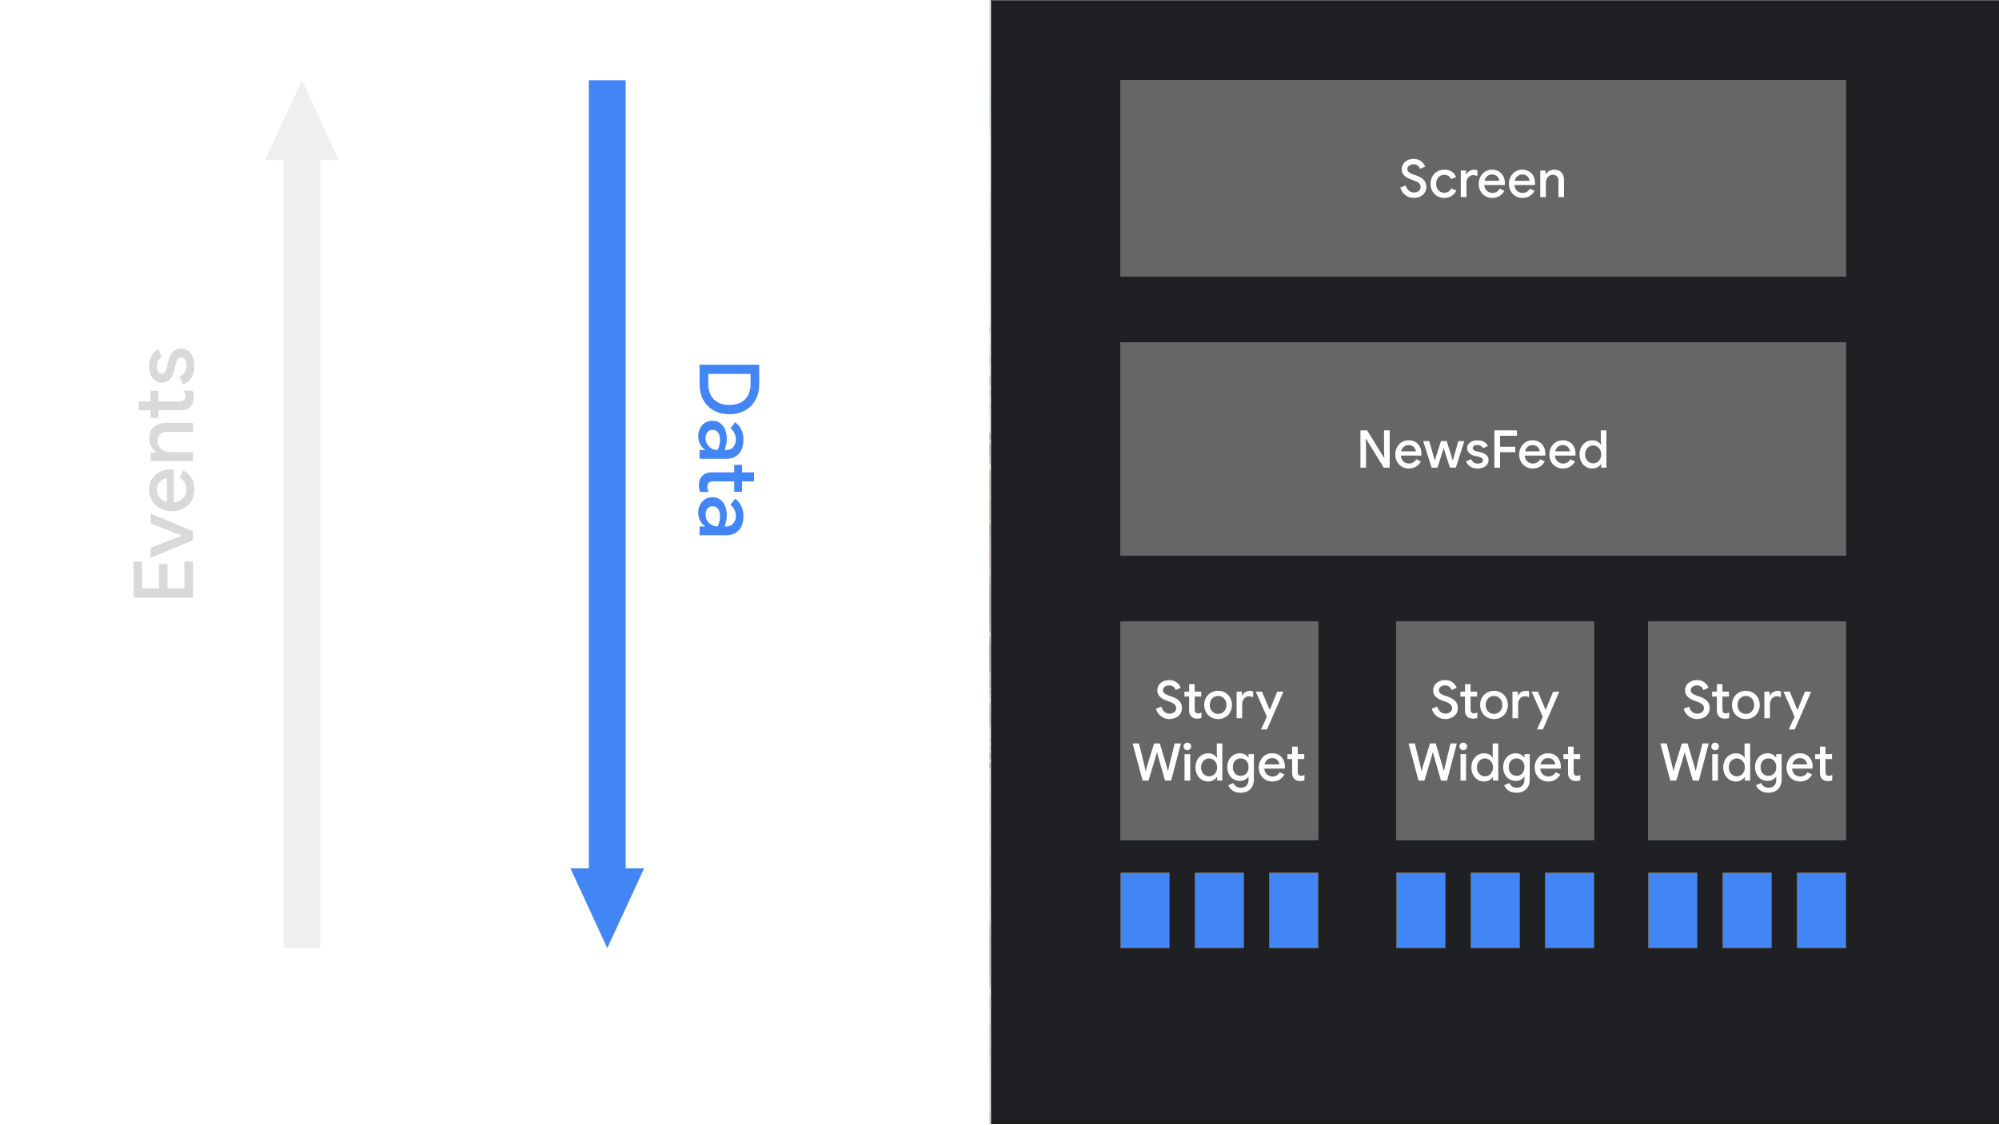
\includegraphics[width=0.9\linewidth]{assets/declarative.png}
    \caption{声明式的编程模型}
    \label{fig:declarative}
\end{figure}

Jetpack Compose采用了声明式的编程模型,这意味着开发者只需描述UI在特定状态下的样子,而不需要明确地指定如何绘制或更新UI。当应用程序的状态发生变化时,Jetpack Compose会自动计算出UI的更新部分,并有效地重新绘制屏幕。这种模型与传统的命令式UI框架(如基于View的Android UI)形成了鲜明对比。

\begin{figure}[htbp]
    \centering
    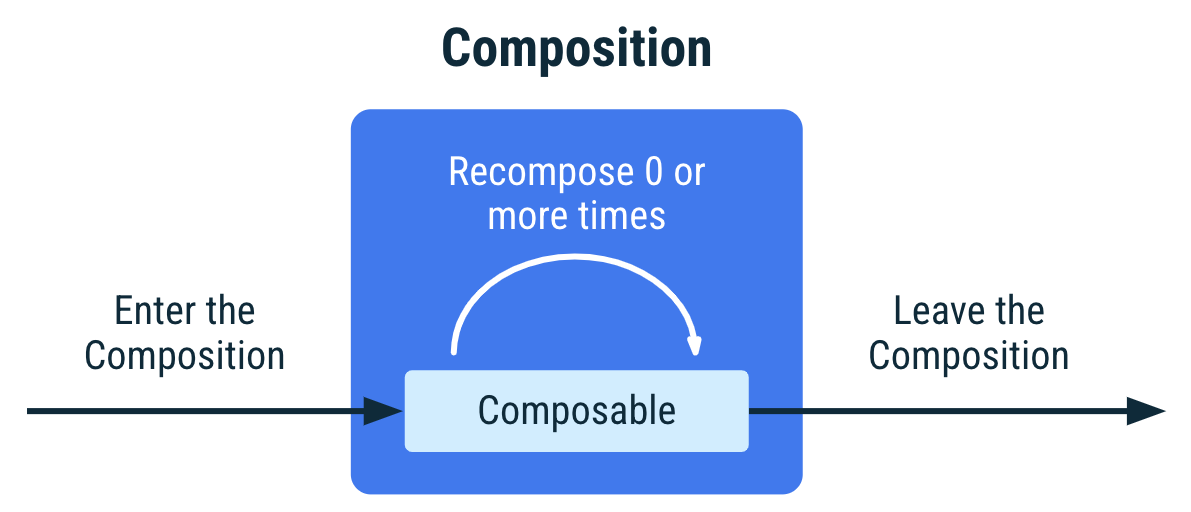
\includegraphics[width=0.9\linewidth]{assets/composition.png}
    \caption{可组合式函数示意}
    \label{fig:composition}
\end{figure}

Jetpack Compose的核心概念是可组合函数(@Composable),这些函数被注解修饰,可以创建和组织UI元素。可组合函数可以嵌套调用,形成复杂的UI布局。它们类似于React中的组件,但更专注于描述UI的局部片段,而非整个组件树。例如对于下面这段代码,其就直接描述了图\ref{fig:compose-example}中的UI树。

\begin{lstlisting}[language=Kotlin]
    @Composable
    fun MyComposable() {
        Column {
            Text("Hello")
            Text("World")
        }
    }
\end{lstlisting}

\begin{figure}
    \centering
    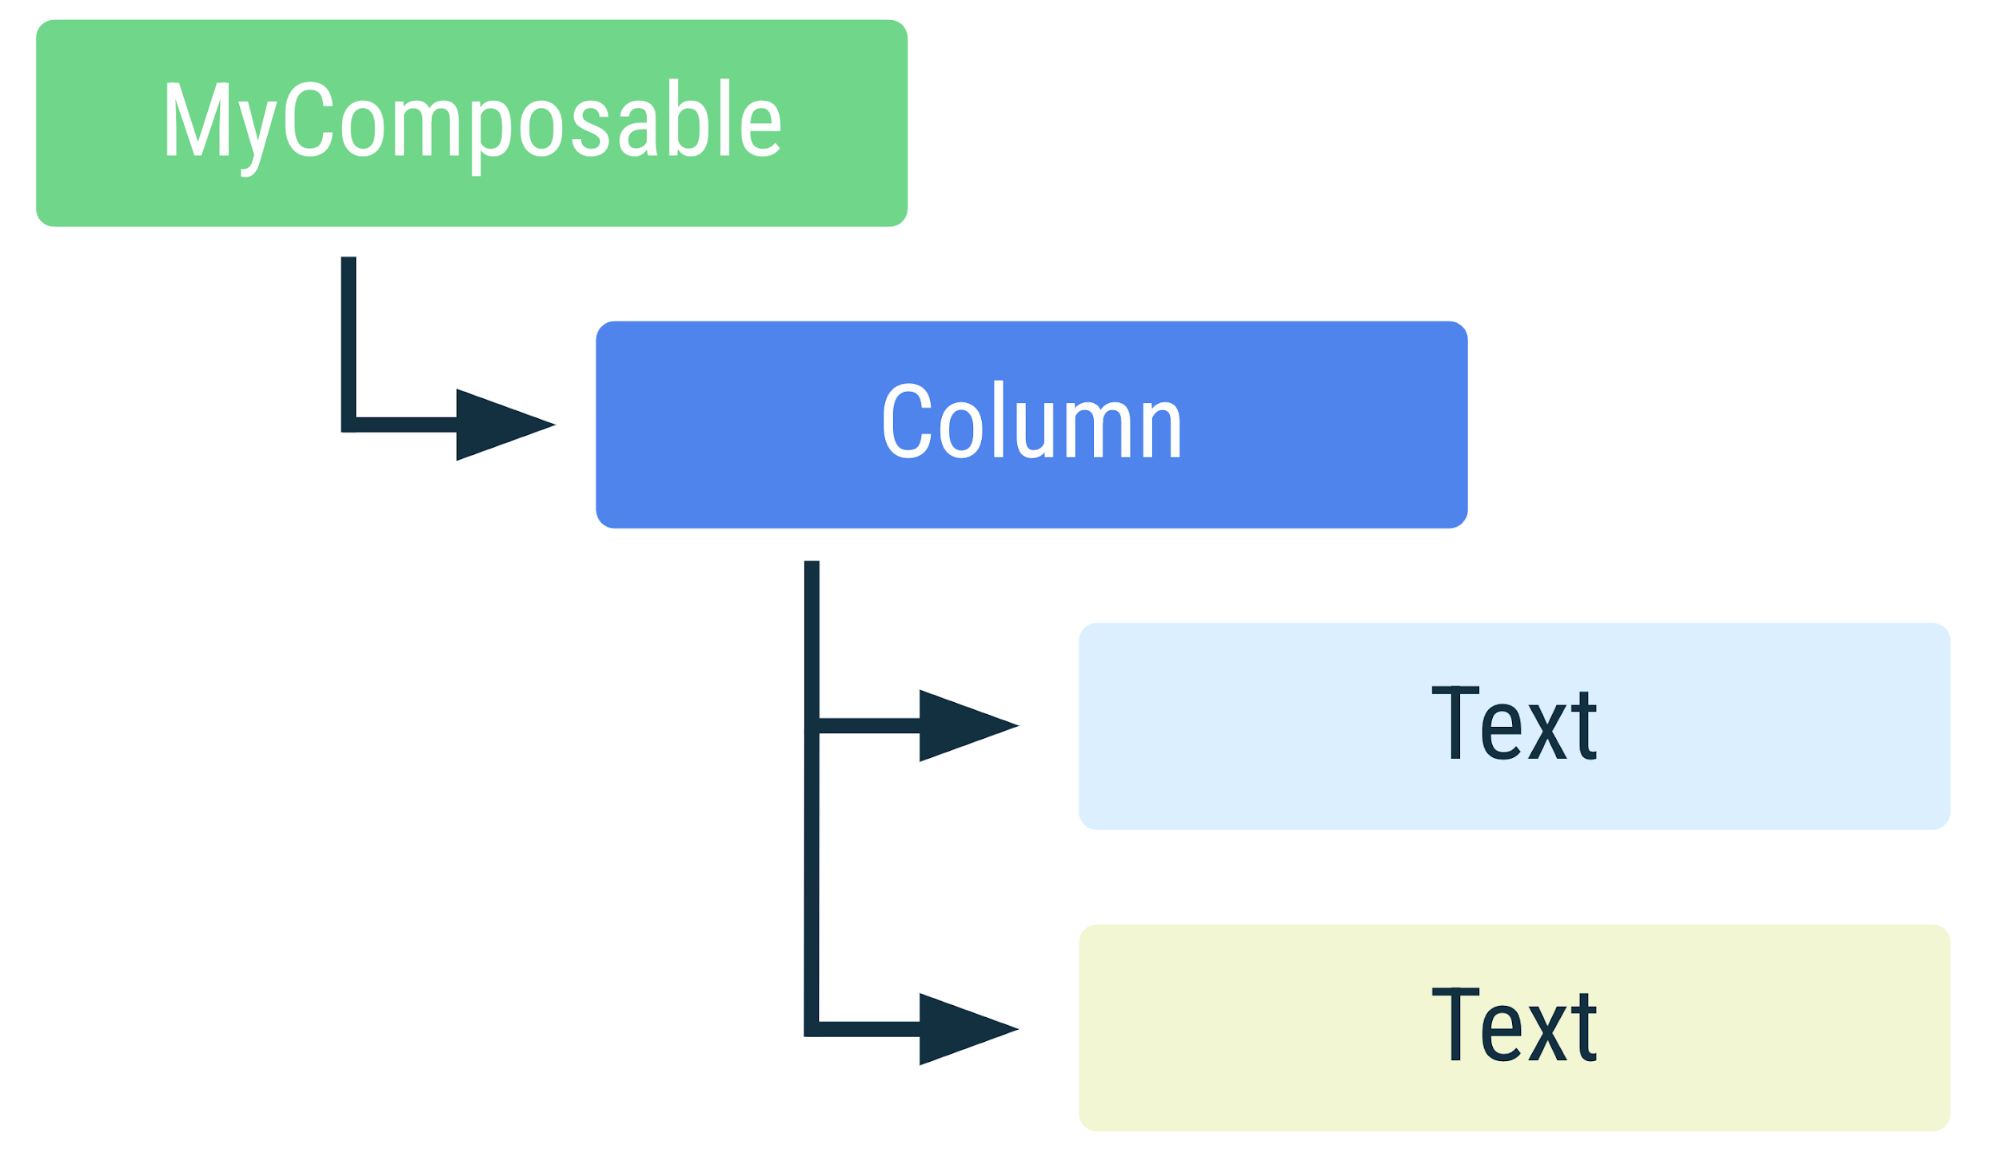
\includegraphics[width=0.9\linewidth]{assets/compose-example.png}
    \caption{MyComposable函数声明的UI树}
    \label{fig:compose-example}
\end{figure}

Jetpack Compose提供了管理状态的机制,包括使用remember和mutableStateOf等函数来存储和更新UI相关的状态。同时,它还提供了处理副作用(如启动动画、发送网络请求)的机制,如LaunchedEffect和DisposableEffect。

Jetpack Compose的很多核心能力,比如将可组合函数转换成有效的UI渲染指令,都是通过Kotlin编译器插件实现的。这些插件在编译阶段处理Composable函数,生成优化过的代码,以提高运行时性能。

Jetpack Compose提供了一套完整的动画API,可以轻松创建复杂的动画效果,包括过渡动画、属性动画和自定义动画。这些动画可以无缝集成到UI的构建过程中,无需额外的动画框架或库。

Jetpack Compose内置了Material Design组件,使得遵循Material Design规范的UI设计变得容易。这些组件包括按钮、文本字段、滑块等,它们可以被直接在可组合函数中使用。

Jetpack Compose使用了被称为\textbf{单向数据流}的软件工程设计模式,特别是前端框架中用于管理组件间数据流动的设计模式。这种模式强调数据的流动是单向的,即数据只沿着一个固定的方向传递,而不是在组件之间来回双向传递。这种模式有助于保持数据流的清晰和可预测性,使得应用的状态更容易理解和维护。

单向数据流模式具有如下的特点。一是数据从父组件传递到子组件,通常通过属性(props)实现。子组件通过这些属性接收数据,并将其用于渲染。二是子组件不能直接修改从父组件接收的数据。如果需要与父组件交互,子组件会触发事件(通常通过回调函数),这些事件携带的信息会被父组件捕获并作出响应。三是对于更复杂的应用,可能需要在更高层次上集中管理状态。这样,组件可以请求更新状态,但状态的变更由中心化的控制器控制,确保数据流的单向性。

使用单向数据流模式对于相对于之前的Android界面设计模型(即允许数据的双向绑定),带来了这些好处:
\begin{itemize}
    \item \textbf{可预测性}:由于数据流的路径是固定的,因此更容易追踪数据变化,预测应用的行为。
    \item \textbf{易于调试}:当数据只沿一个方向流动时,调试问题会更加直接,因为不需要考虑数据的多源头或多目标。
    \item \textbf{模块化}:组件可以独立于其他组件编写和测试,因为它们的输入和输出是明确定义的。
\end{itemize}

\subsection{依赖注入}

依赖注入(Dependency Injection,DI)和控制反转(Inversion of Control,IoC)是软件工程中,特别是在面向对象编程中,用于降低代码耦合度和提高模块间解耦的重要设计模式和原则。

控制反转是一种设计原则,它描述了软件组件控制流的反转。在传统的编程模式下,组件控制着它们的依赖项的创建和生命周期;而在IoC中,这种控制权被“反转”给了外部容器或框架。这意味着组件不再负责初始化和管理其依赖,而是由外部实体(通常是一个框架或容器)来承担这一职责。IoC的目标是降低组件间的耦合,使得各个组件更加独立,易于测试和维护。

依赖注入是实现控制反转的一种常用手段。它是一种设计模式,其中对象的依赖关系不在对象内部创建和管理,而是在对象被创建时由外部实体(如IoC容器)注入。依赖注入有几种不同的形式:

\begin{itemize}
    \item 构造器注入(Constructor Injection):依赖项通过构造函数的参数传递给对象。这是最推荐的方式,因为它可以保证依赖项的不可变性,且易于单元测试。
    \item 属性注入(Property Injection):依赖项通过setter方法或公共属性在对象创建后注入。这在某些情况下可能不太安全,因为依赖项可能在对象使用前没有正确设置。
    \item 方法注入(Method Injection):依赖项通过方法调用在需要的时候注入。这种方法较少见,通常不推荐,因为它可能导致代码的可读性和可维护性下降。
\end{itemize}

依赖项注入为应用的开发带来了如下的优势:

\begin{itemize}
    \item 重用类以及分离依赖项:更容易换掉依赖项的实现。由于控制反转,代码重用得以改进,并且类不再控制其依赖项的创建方式,而是支持任何配置。
    \item 易于重构:依赖项成为 API Surface 的可验证部分,因此可以在创建对象时或编译时进行检查,而不是作为实现详情隐藏。
    \item 易于测试:类不管理其依赖项,因此在测试时,您可以传入不同的实现以测试所有不同用例。
\end{itemize}

在Android开发中,Hilt是一个非常流行的依赖注入框架,它由Google维护,基于Dagger 2构建,但提供了更简化和更易于使用的API,尤其针对Android的开发环境进行了优化。Hilt的主要目标是减少依赖注入所需的样板代码,使得依赖注入更加直观和易于理解。

Hilt主要涉及以下几个概念:
\begin{itemize}
    \item 依赖注入:在软件工程中,依赖注入(Dependency Injection, DI)是一种设计模式,它允许你将依赖项的创建和管理委托给外部实体,而不是在类内部创建。这样可以降低类之间的耦合度,使得代码更易于测试和维护。
    \item 作用域:Hilt支持作用域,这意味着你可以定义依赖项的生命周期。例如,你可能希望在Activity的生命周期内仅创建一次依赖项,或者在整个应用程序的生命周期中共享一个依赖项。
    \item 组件和模块:Hilt使用组件和模块来组织和配置依赖项。组件负责依赖项的创建和管理,而模块则定义了依赖项的绑定规则。
\end{itemize}

\subsection{Jetpack Media3}

Jetpack Media3是Google为Android平台提供的一套多媒体框架,它是Media2的继任者,旨在提供更现代化、更灵活、更强大的媒体播放能力。Media3主要聚焦于音频和视频播放,它包含了一系列的库,旨在帮助开发者更轻松地集成高质量的媒体播放体验到他们的应用中。

\begin{figure}[htbp]
    \centering
    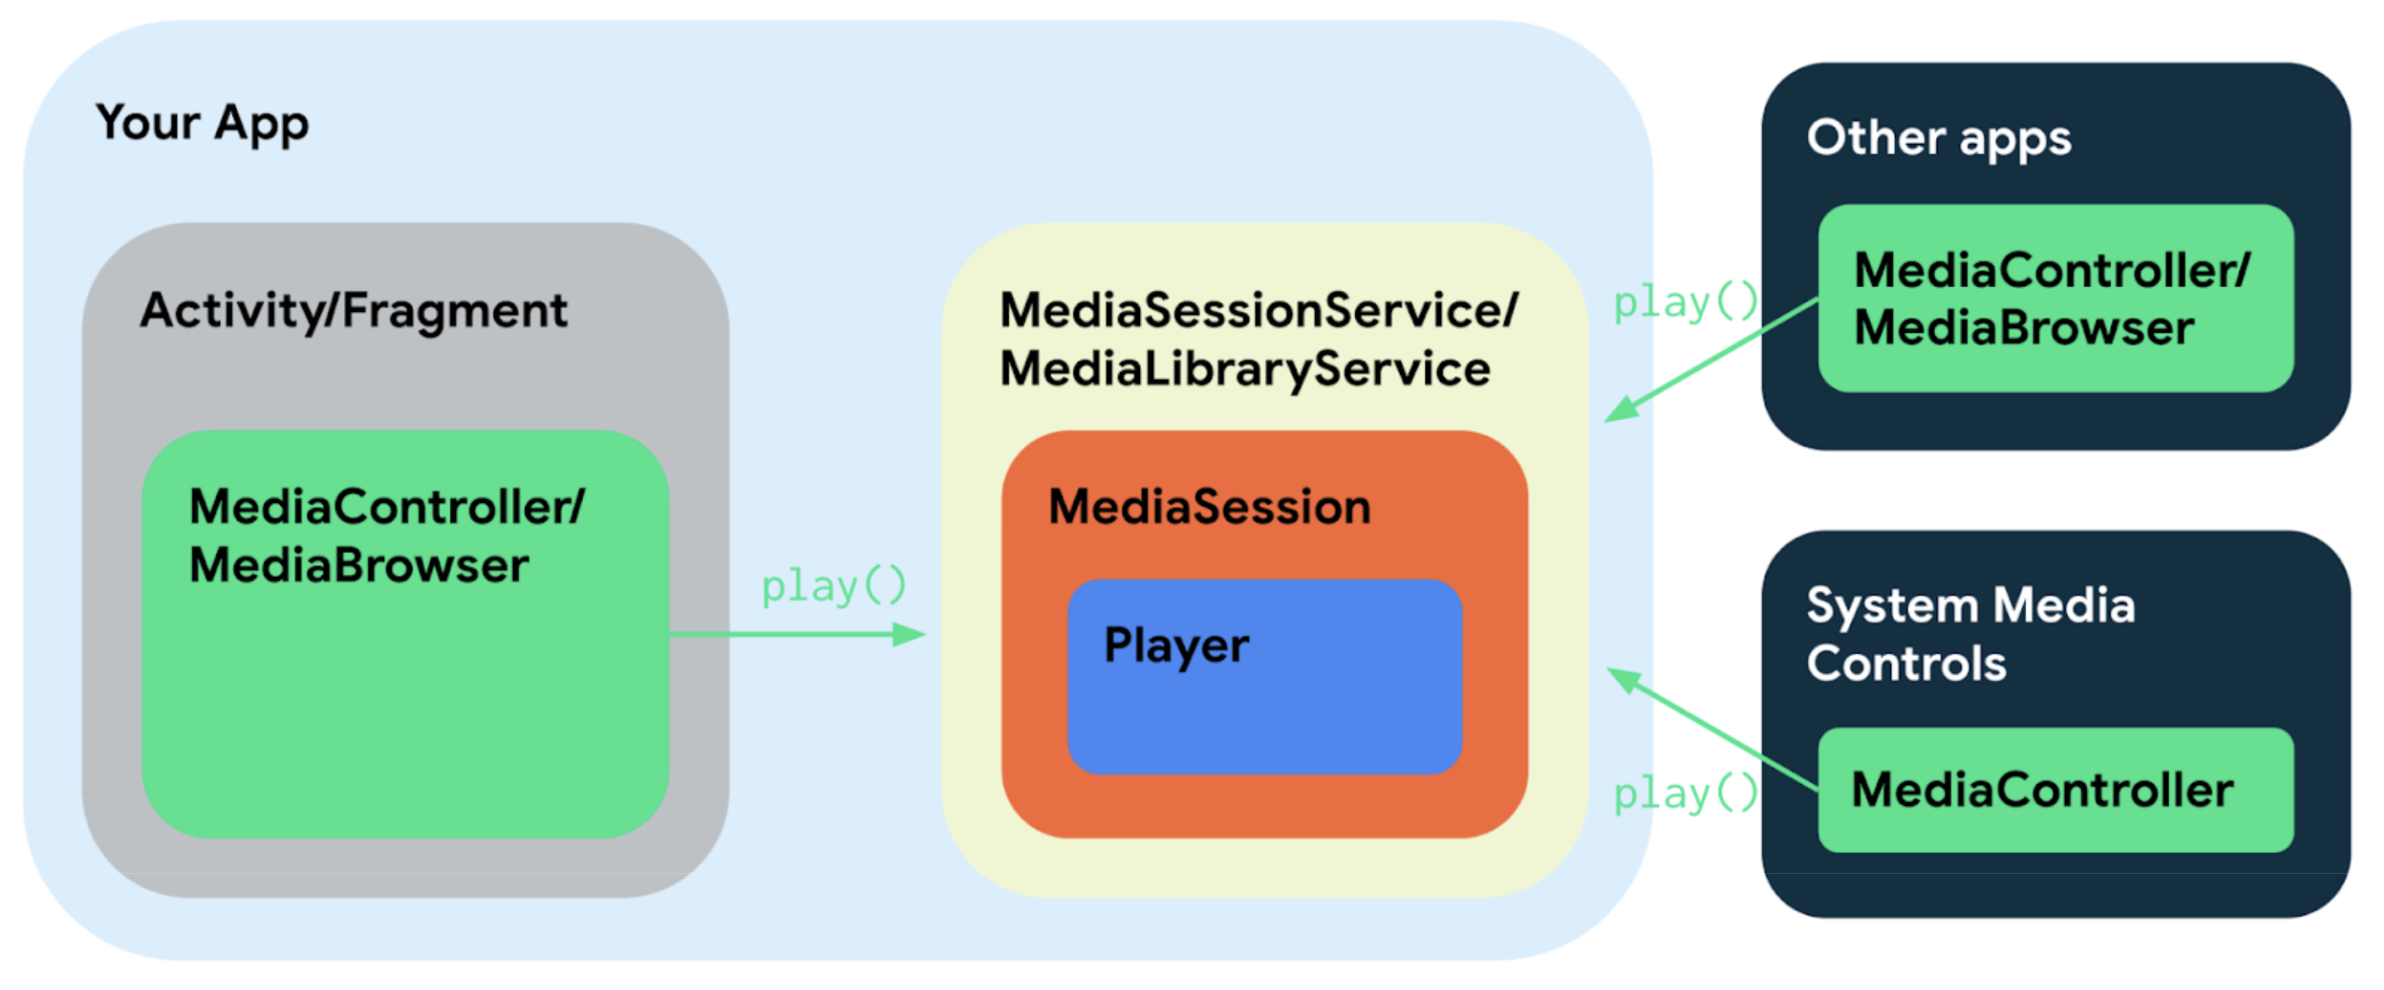
\includegraphics[width=0.9\linewidth]{assets/media-components.png}
    \caption{媒体组件组合示例}
    \label{fig:media-components}
\end{figure}

Media3多媒体框架提供了如下一些特点:
\begin{itemize}
    \item 模块化设计:Media3被设计成一系列模块,这允许开发者根据自己的需求选择和集成特定的组件,比如播放器、数据源、解码器等,而不是被迫使用整个框架。
    \item ExoPlayer集成:Media3的核心是ExoPlayer,这是一个高性能的开源媒体播放器库,能够支持广泛的媒体格式和流媒体协议,如MP4、WebM、FLAC、MP3、AAC、Ogg、TS、WAV等。
    \item API一致性:Media3提供了一致的API,使得开发者可以轻松地在不同的媒体播放场景中切换播放器的实现,而无需大量修改代码。
    \item 向后兼容性:Media3致力于提供向后兼容的API,确保它可以运行在广泛的Android设备上,包括较旧的设备。
    \item 高级功能:Media3支持多种高级功能,如DRM(数字版权管理)、字幕、多音轨、画中画模式、HDR视频等。
    \item 易用性和可定制性:Media3提供了一个易于使用的API,同时也允许开发者深度定制播放器的行为和外观,以满足特定的应用需求。
\end{itemize}

Media3为播放提供了一些关键组件,这些组件大大降低的编写多媒体播放器的复杂度。图\ref{fig:media-components}说明了这些组件在典型应用如何组合在一起。

\paragraph{媒体播放器} 媒体播放器是应用中允许播放媒体文件的组件。

\begin{table*}[htbp]
    \centering
    \begin{tabularx}{\textwidth}{|l|X|X|}
    \hline
    类 & 说明 & 实现注意事项 \\
    \hline
    Player & Player 是一个接口,定义了媒体播放器的传统高级功能,如播放、暂停和跳转功能。& 在 Media3 中,Player 接口是多个组件(例如 MediaSession 和 MediaController)实现或使用的常见 API。\\
    \hline
    ExoPlayer & ExoPlayer 是 Media3 中 Player 接口的默认实现。 & \\
    \hline
    \end{tabularx}
    \caption{媒体播放器组件}
    \label{tab:my_label}
\end{table*}

\paragraph{媒体会话} 媒体会话提供了一种与媒体播放器互动的通用方式。这样,应用就可以向外部来源通告媒体播放,并接收来自外部来源的播放控制请求。

\begin{figure}[htbp]
    \centering
    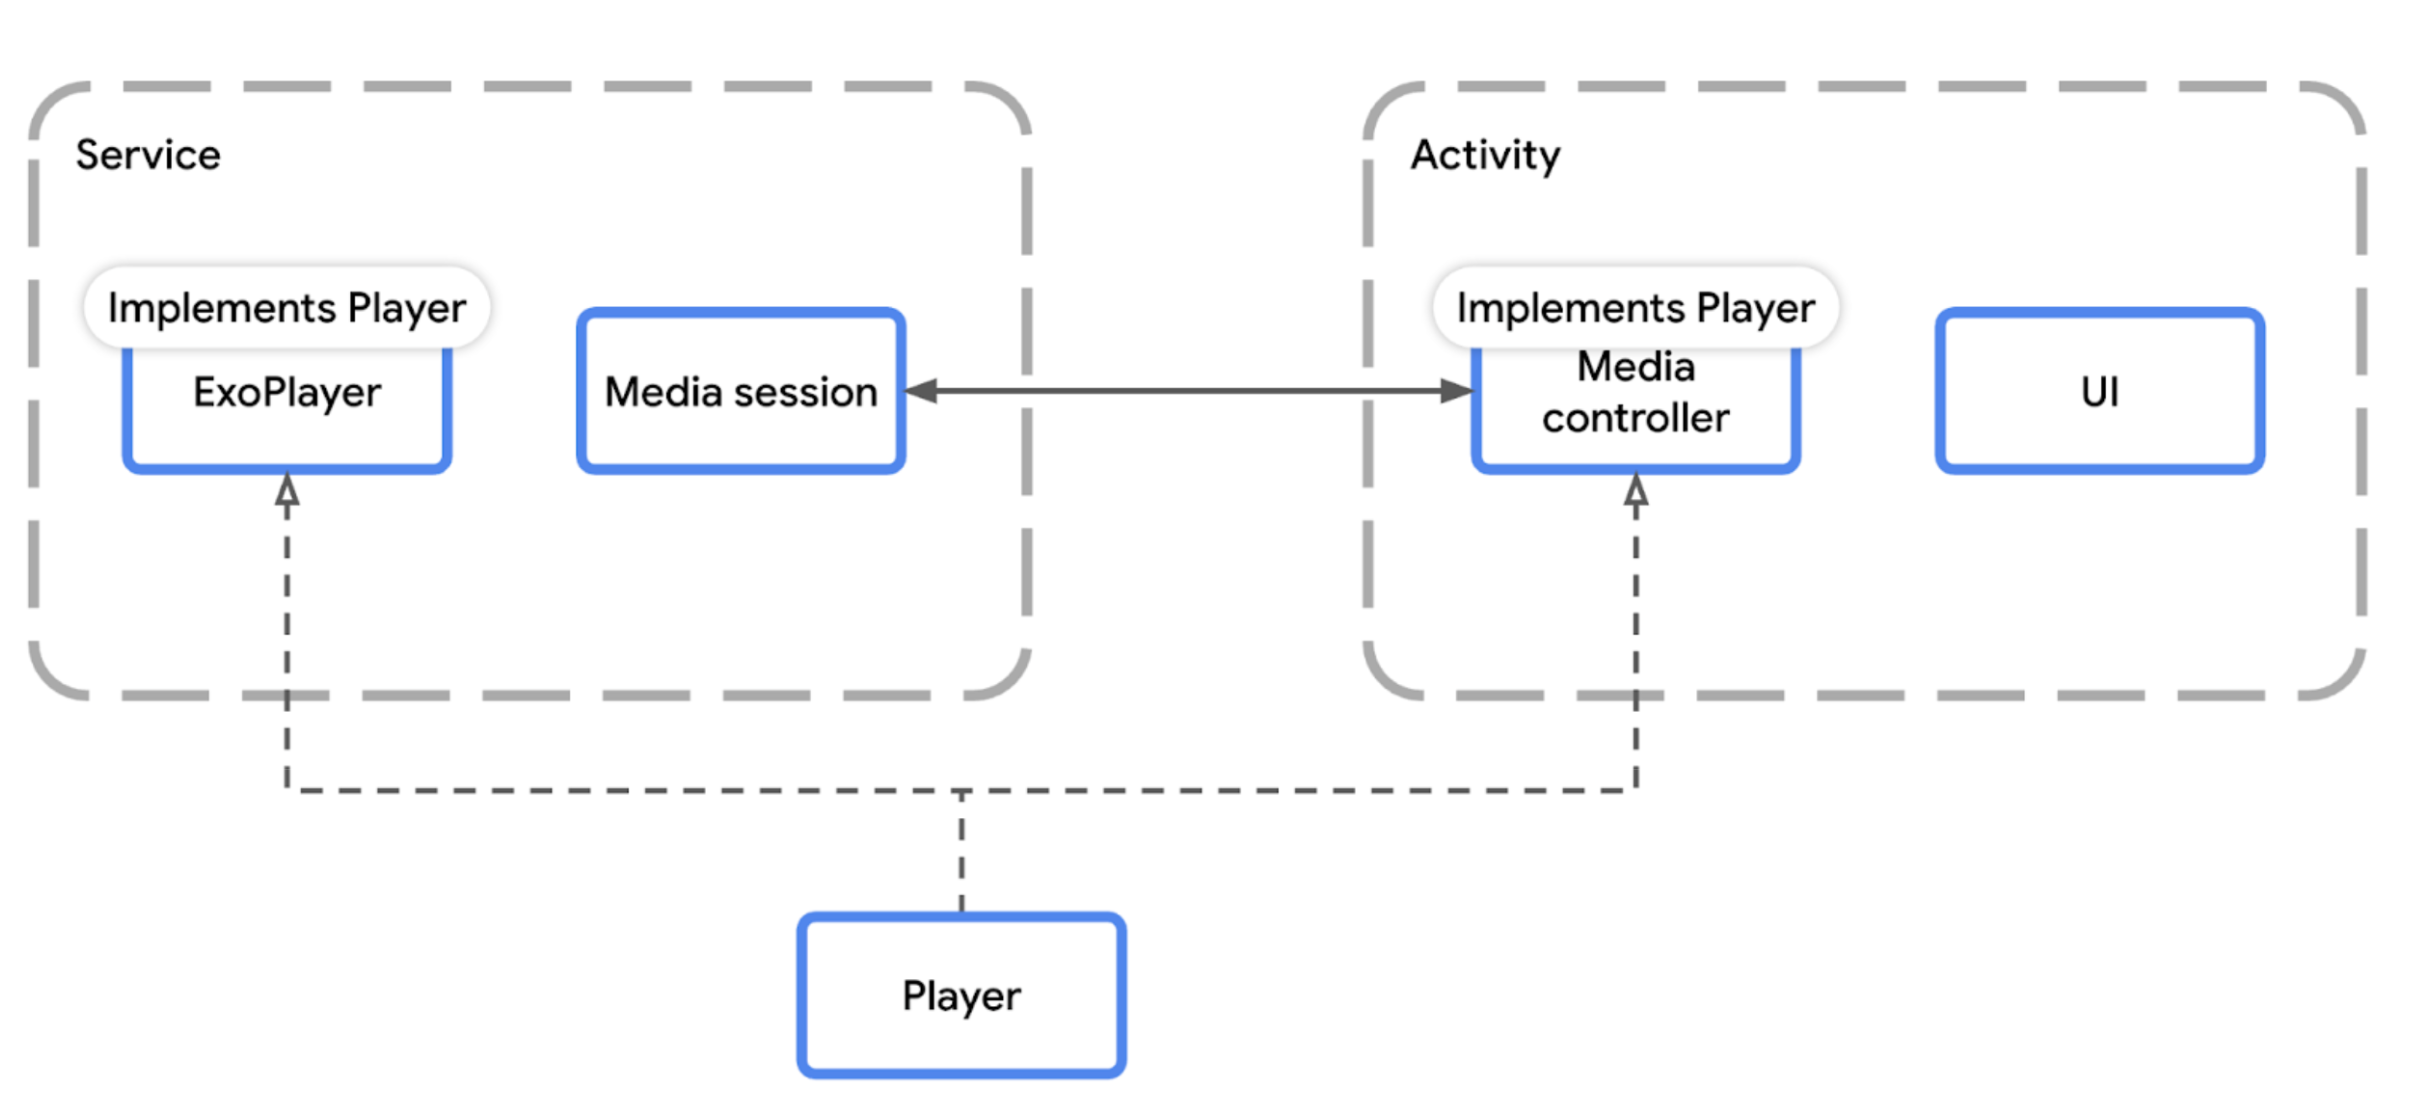
\includegraphics[width=0.9\linewidth]{assets/media3-architecture.png}
    \caption{Media3架构图}
    \label{fig:media-architecture}
\end{figure}

\begin{table*}[htbp]
    \centering
    \begin{tabularx}{\textwidth}{|l|X|X|}
    \hline
    类 & 说明 & 实现注意事项 \\
    \hline
    MediaSession & 媒体会话可让您的应用与音频或视频播放器互动。它们在外部通告媒体播放,并从外部来源接收播放命令。 & 在 Media3 中,MediaSession 需要 Player 才能执行命令并获取当前状态。 \\
    \hline
    MediaSessionService & MediaSessionService 将媒体会话及其关联的播放器保存在与应用的主 Activity不同的服务中,以便于后台播放。 & \\
    \hline
    MediaController & MediaController 类通常用于从应用外部发送命令,例如从其他应用或系统本身发送命令。这些命令会被发送到关联 MediaSession 的底层 Player 。 & MediaController 类实现了 Player 接口,但在调用方法时,该命令会被发送到已连接的 MediaSession。诸如 Google 助理等客户端应用可以使用 MediaController 在已连接的会话中控制播放。 \\
    \hline
    MediaLibraryService & MediaLibraryService 与 MediaSessionService 类似,只不过它包含额外的 API,以便您将内容库提供给客户端应用。& \\
    \hline
    MediaBrowser & 通过 MediaBrowser 类,用户可以浏览媒体应用的内容库,并选择要播放的内容。 & MediaBrowser 类同时实现了 MediaController 和 Player 接口。与 MediaController 类似,Android Auto 等客户端应用通常会实现 MediaBrowser。\\
    \hline
    \end{tabularx}
    \caption{媒体会话组件}
\end{table*}

在实际的开发过程中,媒体会话是完成Activity和Service之间通信的重要组件。首先由于性能的原因,为了保证UI界面的响应性,我们往往会将媒体播放的逻辑放置到一个单独的Service上去运行,这就引入了Activity和Service之间通信的问题,在传统的开发过程中,我们可能需要IBinder或者是Messager来完成进程间的通信,亦或使用广播的方式传递消息。但是在Media3框架中,MediaSession的引入为我们完成了这一系列的任务,从图\ref{fig:media-architecture}中可以很清楚的看出这一关系。

\subsection{HLS}

HLS,全称为HTTP Live Streaming,是由苹果公司提出并开发的一种基于HTTP的流媒体网络传输协议。HLS的主要目的是实现实时音视频流的传输,尤其是在网络条件变化较大的环境中,它能提供流畅且自适应的流媒体播放体验。

HLS具有一下关键特点:
\begin{itemize}
    \item 自适应码率:HLS能够根据网络状况自动调整视频的比特率,这意味着在网络条件不佳时,视频质量会自动降低以保持流畅播放,而在网络良好时,视频质量会提升。
    \item 基于HTTP的传输:使用HTTP作为传输协议,HLS可以利用现有的HTTP基础设施,这使得它易于部署,不需要专门的流媒体服务器硬件。
    \item 媒体文件切片:HLS将媒体内容分割成一系列短小的基于HTTP的媒体片段,每个片段都可以独立下载。这不仅提高了容错能力,还允许快速频道切换。
    \item 清单文件(Playlist):HLS使用一个M3U8格式的文本文件作为清单,其中包含了指向媒体片段的URL链接以及元数据。客户端通过解析这个清单文件来获取并播放媒体片段。
    \item 广泛的支持:HLS不仅被苹果的设备和平台所支持,也被许多其他厂商和流媒体播放器所采纳,包括Android设备、智能电视、游戏机和网页浏览器等。
\end{itemize}

HLS的工作流程通常如下:服务器将视频流切分为多个小的TS(Transport Stream)文件,并生成一个M3U8格式的清单文件。客户端(如iOS设备或Safari浏览器)首先请求M3U8清单文件,然后根据当前网络状况选择合适的比特率流开始播放。当客户端检测到网络状况变化时,它会自动选择不同比特率的流,以维持播放的连续性和流畅性。

\subsubsection{FFmpeg}

FFmpeg是一个极其强大且功能全面的开源软件项目,主要用于处理多媒体数据,包括音频和视频。它被广泛地用于多种场景,如流媒体服务、转码服务、开发多媒体应用以及个人和专业级别的音视频处理任务。

以下是FFmpeg的一些关键特性:

\begin{itemize}
    \item 编码和解码:FFmpeg支持大量的音频和视频编解码器,这使得它可以处理几乎所有的主流格式,从古老的编码方式到最新的编码标准,如H.264、H.265(HEVC)、VP9、AAC、MP3等。
    \item 容器格式:它能够读取和写入多种容器格式,如MP4、AVI、MKV、FLV、TS、MPEG等,这意味着你可以将不同格式的音视频文件转换为其他格式。
    \item 流媒体:FFmpeg可以将音视频流化,支持RTSP、HTTP、RTMP等多种网络协议,使得实现实时流媒体传输成为可能。
    \item 过滤器系统:FFmpeg提供了一套强大的音频和视频过滤器,允许对音视频进行复杂处理,如裁剪、缩放、旋转、颜色调整、去噪、混音等。
    \item GPU加速:它利用硬件加速,如CUDA、OpenCL和VAAPI,来提升视频处理性能。
    \item 跨平台:FFmpeg在各种操作系统上都可以运行,包括Linux、Windows、macOS、BSD和Solaris等。
    \item 库支持:FFmpeg的核心组件包括libavcodec(编解码器库)、libavformat(封装器库)、libavutil(通用工具库)、libavfilter(过滤器库)和libavdevice(设备输入输出库),这些库可以被其他软件集成以实现多媒体处理功能。
    \item 命令行工具:FFmpeg提供了一系列命令行工具,如ffmpeg(用于转换和流化)、ffplay(一个简单的媒体播放器)和ffprobe(用于检查媒体文件的元数据)。
\end{itemize}

在系统中主要涉及到使用FFmpeg生成HLS(HTTP Live Streaming)流涉及到将视频内容分割成一系列较小的HTTP可寻址的文件片段,同时创建一个M3U8索引文件来列出这些片段。下面是系统中使用的命令:

\begin{lstlisting}
ffmpeg -re -i video.mp4 -c:v h264 -f hls -profile:v high10 -hls_list_size 10 -hls_time 10 -hls_base_url /api/hls -hls_flags delete_segments -o output.m3u8
\end{lstlisting}

命令中参数的含义为:

\begin{itemize}
    \item -re: 这个选项让FFmpeg以实时方式读取输入文件,就像从实时源读取数据一样。这在处理实时或流式传输的输入时非常有用,但对于普通的文件输入来说,这个选项可能不是必要的。
    \item -i video.mp4: 指定要转换的输入视频文件为video.mp4。
    \item -c:v h264: 指定视频编码器为H.264。这告诉FFmpeg使用H.264编码器对视频进行编码。
    \item -profile:v high10: 指定H.264编码的配置文件为high10。high10是一个支持10位颜色深度的高级配置文件,通常用于高质量视频,可以提供更细腻的色彩过渡和减少色带效应。
    \item -f hls: 输出格式为HLS (HTTP Live Streaming),这是一种适应性比特率流媒体协议,适用于通过HTTP服务器进行视频流传输。
    \item -hls\_list\_size 10: 指定M3U8播放列表中保留的最新片段数量为10。当新的片段被添加时,最早的那个片段会被删除,保持列表中的片段数量为10。
    \item -hls\_time 10: 设置每个HLS片段的持续时间为10秒。这是HLS片段的默认时长。
    \item -hls\_base\_url /api/hls: 指定HLS片段的基URL为/api/hls。这意味着生成的M3U8播放列表中的每个片段引用都将以前缀/api/hls开始。
    \item -hls\_flags delete\_segments: 添加了一个HLS标志,告诉FFmpeg在片段过期后删除它们。这有助于节省磁盘空间,因为不再需要的旧片段会被自动清理。
    \item -o output.m3u8: 指定输出的M3U8播放列表文件名为output.m3u8。这是HLS流的主要索引文件,客户端会请求这个文件来获取可用的视频片段列表。
    
\end{itemize}

综上所述,这个命令将video.mp4文件转换为HLS格式,使用H.264编码器和high10配置文件进行编码,生成的流将有10个最新的10秒片段,片段的URL将以/api/hls开头,并且过期的片段将会被自动删除。最终的M3U8播放列表文件名为output.m3u8。上述配置是为了实时流媒体服务和需要高质量视频流的应用场景而优化的。

\subsection{OpenAPI}

如何保证前端和后端之间的接口一致性的前后端分离的开发模式中非常重要的一点,在本系统中引入了OpenAPI这一框架来解决这一问题。

OpenAPI(原名Swagger)是一种规范和框架,用于描述API,特别是RESTful API的结构。它提供了一种标准的方式来定义API的行为,包括其路径、参数、模型、响应等,使得API的设计者能够清晰地表达API的功能而无需考虑具体的实现细节。OpenAPI规范使用JSON或YAML格式来描述API,允许开发者、测试人员和API消费者之间进行更有效的沟通和协作。

以下是OpenAPI的一些关键特点和用途:
\begin{itemize}
    \item 标准化:OpenAPI提供了一套标准化的模式,用于描述API接口,使得API文档可读性强,易于理解,同时也有利于自动化工具的生成和消费。
    \item 自动生成文档:基于OpenAPI规范,可以自动生成API的交互式文档,如Swagger UI,这极大地提高了开发效率和用户体验,使开发者能够快速理解和测试API。
    \item 代码生成:OpenAPI还支持从API描述中自动生成服务器端和客户端的代码,支持多种编程语言,如Java、Python、C\#等,从而减少了手动编写代码的工作量,提高了开发效率。
    \item API测试与验证:OpenAPI规范可以用于自动化API测试,因为它提供了API的完整描述,包括所有路径、参数、响应等,这使得编写测试用例变得简单和直接。
    \item API发现与注册:OpenAPI规范还可以用于API的发现和注册,使得API能够在一个组织内或跨组织间被轻松查找和复用。
    \item 生态系统:围绕OpenAPI已经形成了一个丰富的工具和社区生态系统,包括编辑器、IDE插件、代码生成器、测试工具等,这些工具和服务进一步增强了OpenAPI的价值。
\end{itemize}

openapi-generator是一个强大的工具,可以基于OpenAPI (Swagger) 规范自动生成服务器存根和客户端库的源代码。openapi-generator的Gradle插件允许你在构建过程中集成代码生成,这样可以自动化地保持你的代码与API规范同步。在系统中使用openapi-generator和Gradle相配合的情况下从后端生成的接口文档中生成前后端通信的胶水代码。在Android项目中使用openapi-generator的过程简述如下:

首先在build.gradle.kts文件中添加openapi-generator插件依赖。

\begin{lstlisting}[language=Kotlin]
plugins {
    // other plugins
    alias(libs.plugins.openapi.generator)
}
\end{lstlisting}

接下来,在build.gradle.kts中配置openapi-generator插件。这通常涉及到指定API规范的位置以及想要生成的目标语言和输出目录。在系统中的配置代码为:

\begin{lstlisting}[language=Kotlin]
openApiGenerate {
    generatorName.set("kotlin")
    inputSpec.set("$rootDir/app/src/main/openapi/chiara.json")
    outputDir.set(openapiOutputDir)
    apiPackage.set("top.rrricardo.chiara.openapi.api")
    modelPackage.set("top.rrricardo.chiara.openapi.model")
    packageName.set("top.rrricardo.chiara.openapi.client")
    generateApiTests.set(false)
    generateModelTests.set(false)
    configOptions.set(
        mapOf(
            "dataLibrary" to "java8"
        )
    )
    additionalProperties.set(
        mapOf(
            "library" to "jvm-retrofit2",
            "serializationLibrary" to "kotlinx_serialization",
            "useCoroutines" to "true",
        )
    )
}
\end{lstlisting}

保存build.gradle更改后,在命令行中运行以下命令来执行代码生成:

\begin{lstlisting}
./gradlew openApiGenerate
\end{lstlisting}

这将会根据输入的OpenAPI规范文件生成代码,并将其放置在指定的输出目录中。一旦生成了代码,将它整合到你的项目中,这需要修改build.gradle.kts文件中对于\texttt{android}进行配置:

\begin{lstlisting}[language=Kotlin]
    sourceSets["main"].kotlin {
        srcDir("$openapiOutputDir/src/main/kotlin")
    }
\end{lstlisting}

在使用代码生成的过程中,需要注意:

\begin{enumerate}
    \item 确保你的OpenAPI规范是最新的,以便生成的代码能够正确反映API的状态。
    \item 定期运行代码生成任务,特别是在API规范发生改变时,以保持生成的代码与规范同步。
    \item 如果你需要生成不同语言的代码或者有多个规范文件,你可以在build.gradle.kts中定义多个openApiGenerate任务,每个任务对应一个不同的规范和生成配置。
\end{enumerate}

\end{document}